%%% Преамбула ГОСТ 7.32
%%% Артемий Владин
%%% https://github.com/temavladin


%% Формат бумаги, размер шрифта (12pt или 14pt)
%% documentclass a4paper 14pt extarticle


%% Локализация
\usepackage[english,russian]{babel}
\usepackage{indentfirst} %% Красная строка
\addto\captionsrussian{\renewcommand{\figurename}{Рисунок}}
\addto\captionsrussian{\renewcommand{\tablename}{Таблица}}
\addto\captionsrussian{\renewcommand{\contentsname}{\hfill \normalsize \bfseries СОДЕРЖАНИЕ \hfill}}


%% Основной шрифт
\usepackage{fontspec}
\setmainfont[Ligatures=TeX]{Times New Roman}

%% Машинописный шрифт
\setmonofont{Courier New}
%\setmonofont{Consolas}[Scale=0.9]
%\setmonofont{Fira Mono}

%% Математический шрифт (Рекомендуемые: STIX или XITS)
\usepackage{mathtools}
\usepackage[warnings-off={mathtools-colon,mathtools-overbracket}]{unicode-math}
%\setmathfont{STIX Two Math}
%\setmathfont{STIX Two Math}[range={it/greek->up,bfit/greek->bfup}]


%% Поля документа
\usepackage[left=30mm, right=15mm, top=20mm, bottom=20mm]{geometry}
%% Нумерация страниц
\pagestyle{plain}

%% Абзацный отступ
\setlength{\parindent}{1.25 cm}
%% Межабзацный интервал
\setlength{\parskip}{0pt}

\usepackage{setspace}
%% Полуторный межстрочный интервал
\onehalfspacing


%% Настройка переноса слов
\usepackage{microtype}
\pretolerance=-1 %% Отключение попытки выравнивания строки без переносов
\tolerance=300 %% Позволяет избежать длинных пробелов
\emergencystretch=3em %% Аварийное растяжение межсловных пробелов
\exhyphenpenalty=150 %% Штраф для переносов после дефиса
\doublehyphendemerits=10000 %% Запрет на два переноса подряд в двух соседних строках
\finalhyphendemerits=10000 %% Запрет переноса слова в предпоследней строке абзаца

%% Отключение переноса слов
%\tolerance=1 %% Допуск на разряжённость
%\emergencystretch=\maxdimen %% Растяжение межсловных пробелов
%\hyphenpenalty=10000 %% Запрет на переносы слов
%\hbadness=10000 %% Мера разряжённости


%% Введение рисунков
\usepackage{graphicx}
%% Плавающие объекты
\usepackage{float}
%% Подключение цветов
\usepackage{xcolor}
%% Настройка подписей
\usepackage{subfig}


%% Подключение подписей к объектам
\DeclareCaptionLabelFormat{gost}{#1~#2} %% Формат метки: "Рисунок 1", "Таблица 2"
\DeclareCaptionLabelSeparator{gost}{~---~} %% Разделитель между меткой и текстом подписи
\usepackage{caption} %% Подписи к плавающим объектам

%% Рисунки по центру без переносов
\DeclareCaptionFormat{gost-figure}{%
\begingroup
\centering
\hyphenpenalty=10000
\exhyphenpenalty=10000
#1#2#3%
\endgroup
}

%% Таблицы слева без переносов
\DeclareCaptionFormat{gost-table}{%
\begingroup
\raggedright
\hyphenpenalty=10000
\exhyphenpenalty=10000
#1#2#3%
\endgroup
}

\captionsetup*[figure]{format=gost-figure, labelformat=gost, labelsep=gost}
\captionsetup*[table]{format=gost-table, labelformat=gost, labelsep=gost, singlelinecheck=false}


%% Стили заголовков
\usepackage{xparse} %% Создание своих команд
\NewDocumentCommand{\gostheading}{s m}{ %% Команда для заголовка по ГОСТ
\clearpage
\IfBooleanTF{#1}
{% Звёздочка ЕСТЬ: просто печатаем заголовок (без добавления в содержание)
\begin{center}
\bfseries\MakeUppercase{#2}
\end{center}
}
{% Звёздочки НЕТ: добавляем в оглавление и создаём якорь
\phantomsection
\addcontentsline{toc}{section}{#2}
\begin{center}
\bfseries\MakeUppercase{#2}
\end{center}
}
\par
}


%% Стили заголовков
\usepackage{titlesec}
\titleformat{\section}[hang]
{\normalsize \bfseries \hyphenpenalty=10000} %% Формат
{\thesection}{1 em} %% Нумерация и отступ
{} %% Любой доп. код

\titleformat{\subsection}[hang]
{\normalsize \bfseries \hyphenpenalty=10000}
{\thesubsection}{1 em}
{}
	
\titleformat{\subsubsection}[hang]
{\normalsize}
{\thesubsubsection}{1 em}
{}

%% Отступы от заголовка
\titlespacing*{\section}{12.5 mm}{0.5\baselineskip}{0.1\baselineskip}
\titlespacing*{\subsection}{12.5 mm}{0.5\baselineskip}{0.1\baselineskip}
\titlespacing*{\subsubsection}{12.5 mm}{\parskip}{-\parskip}


%% Настройки содержания
\usepackage{titletoc}

\titlecontents{section}
[2 em] % Общий отступ от левого края
{\vspace{0.3\baselineskip}} % Вертикальный промежуток 
{\contentslabel{2 em}} % Нумерованные
{\hspace*{-2 em}} % Ненумерованные
{\titlerule*[0.5pc]{.}\contentspage} % Точки

\titlecontents{subsection}
[4.9 em]
{}
{\contentslabel{2.7em}}
{\hspace*{2.7em}}
{\titlerule*[0.5pc]{.}\contentspage}

\titlecontents{subsubsection}
[8.6 em]
{}
{\contentslabel{3.5 em}}
{\hspace*{3.5 em}}
{\titlerule*[0.5pc]{.}\contentspage}


%% Стиль списков
\usepackage{enumitem}
\AddEnumerateCounter{\asbuk}{\@asbuk}{\cyrm}
%% Списки начинаются с красной строки (12.5 мм)
\setlist[itemize]{wide=\parindent, leftmargin=*, label={---}, itemsep=0pt, topsep=0pt, parsep=0pt, partopsep=0pt}
\setlist[enumerate]{wide=\parindent, leftmargin=*, itemsep=0pt, topsep=0pt, parsep=0pt, partopsep=0pt}
\setlist[enumerate,1]{label=\arabic*.}
\setlist[enumerate,2]{label=\asbuk*)}


%% Гиперссылки
\usepackage{hyperref}
\hypersetup{
unicode,
colorlinks,
citecolor=black,
filecolor=black,
linkcolor=black,
urlcolor=blue %% Ссылки в интернет синие
}


%% Настройка таблиц
\renewcommand{\arraystretch}{1.3} %% Высота строк таблицы
%\setlength{\tabcolsep}{1 em} % Отступы слева и справа от содержимого ячейки


%% Авто датировка
\usepackage[ddmmyy]{datetime} %% Дата \today
\renewcommand{\dateseparator}{.} %% Разделитель точка


%% Дополнительные пакеты
\usepackage{amsmath, amsthm, amsfonts} %% Математика формулы
%\usepackage{amssymb} %% Этот пакет не работает вместе с unicode-math
\usepackage{icomma} %% Умная запятая для чисел
\usepackage{textcomp}
\usepackage{tabularray}
\usepackage{rotating}
\usepackage{tabularx}
\usepackage{array}
\usepackage{ragged2e}
\usepackage{makecell} %% Переносы в клетках таблицы
\usepackage{hhline} %% Улучшенные горизонтальные линии в таблицах
\usepackage{multirow} %% Ячейки в несколько строчек в таблицах
\usepackage{longtable} %% Многостраничные таблицы


%% Листинг
\usepackage{fvextra} %% Улучшенный Verbatim


%% Настройка библиографии
\makeatletter

% 1. Переопределяем окружение thebibliography, чтобы убрать заголовок
\renewenvironment{thebibliography}[1]{
	\par % начинаем с нового абзаца
	\setcounter{mybibcntr}{0} % сбрасываем счетчик источников
}{
	\par % заканчиваем абзацем
}

% 2. Переопределяем команду \bibitem для вывода "Цифра. Текст" как абзац
\newcounter{mybibcntr}
\renewcommand{\bibitem}[1]{%
	\stepcounter{mybibcntr}%
	\par % каждый источник начинается с нового абзаца (будет стандартный отступ 1.25 см)
	% Записываем номер в aux-файл, чтобы команда \cite{} в тексте работала корректно
	\if@filesw \immediate\write\@auxout{\string\bibcite{#1}{\the\c@mybibcntr}}\fi
	\the\c@mybibcntr. \ignorespaces % выводим "1. " и игнорируем пробел после команды
}

\makeatother


%% Приложение ГОСТ
%% Счётчик приложений
\newcounter{gostappendix}
\renewcommand{\thegostappendix}{%
\ifcase\value{gostappendix}%
\or А\or Б\or В\or Г\or Д\or Е\or Ж\or И\or К%
\or Л\or М\or Н\or П\or Р\or С\or Т\or У\or Ф%
\or Х\or Ц\or Ч\or Ш\or Щ\or Э\or Ю\or Я%
\else ?\fi
}

%% Команда для приложения
\NewDocumentCommand{\gostappendix}{m}{%
\stepcounter{gostappendix}%
\clearpage
\phantomsection
	
% Сбрасываем счётчики для нового приложения
\setcounter{section}{0}%
\setcounter{figure}{0}%
\setcounter{table}{0}%
\setcounter{equation}{0}% % Формулы тоже по ГОСТу нумеруются в приложениях
	
% Задаём новый формат нумерации с буквой приложения
\renewcommand{\thesection}{\thegostappendix.\arabic{section}}%
\renewcommand{\thefigure}{\thegostappendix.\arabic{figure}}%
\renewcommand{\thetable}{\thegostappendix.\arabic{table}}%
\renewcommand{\theequation}{\thegostappendix.\arabic{equation}}%

\addcontentsline{toc}{section}{Приложение~\thegostappendix\ --- #1}%
\begin{center}
{\normalsize\bfseries ПРИЛОЖЕНИЕ~\thegostappendix\par}
{\bfseries #1\par}
\end{center}
}


%% Титульный лист
%% Определение заполнителей титульного листа
\newcommand{\UniversityDepartment}[1]{\gdef\setUniversityDepartment{#1}}
\newcommand{\setUniversityDepartment}{}
\newcommand{\TeacherPosition}[1]{\gdef\setTeacherPosition{#1}}
\newcommand{\setTeacherPosition}{}
\newcommand{\TeacherName}[1]{\gdef\setTeacherName{#1}}
\newcommand{\setTeacherName}{}
\newcommand{\WorkNumber}[1]{\gdef\setWorkNumber{#1}}
\newcommand{\setWorkNumber}{}
\newcommand{\WorkName}[1]{\gdef\setWorkName{#1}}
\newcommand{\setWorkName}{}
\newcommand{\UniversityDiscipline}[1]{\gdef\setUniversityDiscipline{#1}}
\newcommand{\setUniversityDiscipline}{}
\newcommand{\StudentGroup}[1]{\gdef\setStudentGroup{#1}}
\newcommand{\setStudentGroup}{}
\newcommand{\StudentName}[1]{\gdef\setStudentName{#1}}
\newcommand{\setStudentName}{}
\newcommand{\DATE}[1]{\gdef\setDATE{#1}}
\newcommand{\setDATE}{\today}


\UniversityDepartment{№ номер}
\TeacherPosition{должность}
\TeacherName{И.О. Фамилия}
\WorkNumber{№ 1}
\WorkName{Название}
\UniversityDiscipline{Дисциплина}
\StudentGroup{ГРУППА}
\StudentName{И.О. Фамилия}
\DATE{\today}

\begin{document}


%%% Пример. Титульный лист для отчёта о НИР по ГОСТ 7.32-2017
%%% Артемий Владин
%%% https://github.com/temavladin


\thispagestyle{empty}

\begingroup
\fontsize{12}{14.4}\selectfont

\begin{center}
Министерство науки и высшего образования Российской Федерации

Федеральное государственное бюджетное научное учреждение

«НАУЧНО-ИССЛЕДОВАТЕЛЬСКИЙ ИНСТИТУТ ЧАРОДЕЙСТВА И ВОЛШЕБСТВА»

(ФГБНУ «НИИЧАВО»)
\end{center}

\vspace{\baselineskip}
\begin{flushleft}
УДК 025.441.47.02(047.31)

Рег. № НИОКТР 114120470044

Рег. № ИКРБС
\end{flushleft}

\vspace{\baselineskip}
\mbox{}\hfill
\begin{minipage}{0.4\linewidth}
УТВЕРЖДАЮ

Директор НИИЧАВО

\rule{6em}{.4pt} Я.П. Невструев

«\rule{2em}{.4pt}» \rule{5em}{.4pt} \the\year{} г.
\end{minipage}

\vspace{\baselineskip}
\begin{center}
ОТЧЕТ

О НАУЧНО-ИССЛЕДОВАТЕЛЬСКОЙ РАБОТЕ

\vspace{\baselineskip}

Примеры оформления структурных элементов и содержания в ЛаТеХ.

Создание отчета с использованием ЛаТеХ-преамбулы Владина

по теме:

ПРИМЕР ОФОРМЛЕНИЯ ОТЧЕТА ПО ГОСТ 7.32-2017 В СИСТЕМЕ LATEX

(промежуточный, этап 1)
\end{center}

\vfill
\begin{flushleft}
Руководитель НИР,

зам. директора по научной работе \hspace{1.5cm} \rule{3cm}{.4pt} Ф.С. Киврин
\end{flushleft}

\vfill

\begin{center}
Санкт-Петербург \the\year{}
\end{center}

\endgroup


\gostheading*{Список исполнителей}

\noindent\begin{tabular}{>\raggedright b{0.43\textwidth} !{\rule{0.21\textwidth}{0.4pt}} >\raggedright p{0.27\textwidth}}

Руководитель НИР, \linebreak зам. директора по научной работе, д-р филол. наук & М.А. Берлиоз \linebreak \footnotesize (введение, заключение) \tabularnewline

Отв. исполнитель, \linebreak зав. отделом, \linebreak канд. ист. наук & И.Н. Понырёв \linebreak \footnotesize (раздел 1, 2, 3) \tabularnewline

Исполнители: \linebreak Ведущий инженер & Ф.Ф. Коровьев \linebreak \footnotesize (раздел 1, 2, 3) \tabularnewline

Нормоконтроль & К.К. Бегемот

\end{tabular}


\gostheading*{Реферат}

Отчёт 20 с., 1 кн., 1 рис., 2 табл., 2 источн., 3 прил.

\noindent ПРИМЕР ОТЧЕТА, ШАБЛОН ОТЧЕТА, СТРУКТУРА ОТЧЕТА, ЛАТЕХ ПРЕАМБУЛА, НАСТРОЙКИ LATEX, ОФОРМЛЕНИЕ ОТЧЕТА

Этот документ показывает внешний вид отчёта, оформленного по ГОСТ 7.32-2017 в системе ЛаТеХ с помощью преамбулы Владина.

Актуальные версии ЛаТеХ-преамбулы и шаблона Владина, а также рекомендации по их использованию можно найти на следующих платформах:

GitHub: \url{https://github.com/temavladin}

Telegram: \url{https://t.me/temavladin}

ВКонтакте: \url{https://vk.ru/temavladin}

Если вам понравился этот проект, поделитесь им с друзьями и подпишитесь на мои соцсети. Вы можете написать мне в ВК или на электронную почту tema@vladin.ru

Отчёт содержит текст-заполнитель, не имеющий смысла. Это просто пример содержания, не воспринимайте текст всерьёз.


\clearpage
\tableofcontents


\gostheading*{Термины и определения}

В настоящем отчете о НИР применяют следующие термины с соответствующими определениями:

\begin{tabular}{p{0.2\textwidth}!{---}p{0.65\textwidth}}
Гравицаппа & деталь от двигателя пепелаца, необходимая для космических полётов \\
Сепульки & наиважнейший элемент цивилизации ардритов. Своей цветовой гаммой напоминают мягкие пчмы \\
Термин & определение \\
Term & definition \\
\end{tabular}


\gostheading*{Перечень сокращений и обозначений}

В настоящем отчете о НИР применяют следующие сокращения и обозначения:

\begin{tabular}{p{0.2\textwidth}!{---}p{0.65\textwidth}}
ГОСТ & государственный стандарт \\
Обозначение & детальная расшифровка \\
Титилипоня & трест изготовления типично интеллектуальной липы по объяснению необъяснимых явлений \\
Abbreviation & detailed explanation \\
\end{tabular}


\gostheading{Введение}

В ЛаТеХ вот таким простым образом можно набирать текст и этот текст будет верстаться в абзацы по установленным в преамбуле настройкам на листы А4 в PDF-документ.

Это введение, здесь нужно написать цели, задачи, актуальность проблемы, исходные данные и так далее, ну, в общем, вы знаете.

Вот смотрите как в ЛаТеХ оформляются списки и перечни:

\begin{enumerate}
	\item Список нумерованный.
	\item Список нумерованный.
	
	\begin{enumerate}
		\item Список нумерованный.
		\item Список нумерованный.
		
		\begin{itemize}
			\item Элемент 1.
			\item Элемент 2.
		\end{itemize}
	\end{enumerate}
\end{enumerate}

Ещё какой-то важный текст:

\begin{itemize}
	\item список маркированный;
	\item список маркированный;
	\item список маркированный.
\end{itemize}

Таким образом, например, вы можете оформить свой список целей и задач.


\clearpage
\section{Заголовок раздела}

\subsection{Заголовок подраздела}

Текст подраздела. Как видите таким образом оформляются заголовки.

\subsubsection{Заголовок пункта}

Текст пункта. Пу-пу-пу...


\clearpage
\section{Всякие штучки в тексте}

\subsection{Примечания}

В тексте можно с лёгкостью добавлять примечания. Непонятка\footnote{Текст примечания}.

\subsection{Ссылки на литературу}

В тексте можно ссылаться на список источников.

Как было сказано в \cite{ivanov2020} вот так и оформляется ссылка.

\subsection{Добавление формул}

Формулы и математические символы можно писать прям внутри строки, например так: $ \alpha+\lambda=\gamma$. Далее продолжать текст и например рассказывать о переменных. $\lambda$ --- буква лямбда.

А можно оформлять и другими способами например как в формуле \eqref{formula}.

\begin{equation}\label{formula}
	x = a_0 + \cfrac{1}{a_1 
		+ \cfrac{1}{a_2 
			+ \cfrac{1}{a_3 + \cfrac{1}{a_4} } } }
\end{equation}

Или например без нумерации можно оформить математику как выключенную из текста формулу:
\[ A_{m,n} = 
\begin{pmatrix}
	a_{1,1} & a_{1,2} & \cdots & a_{1,n} \\
	a_{2,1} & a_{2,2} & \cdots & a_{2,n} \\
	\vdots  & \vdots  & \ddots & \vdots  \\
	a_{m,1} & a_{m,2} & \cdots & a_{m,n} 
\end{pmatrix} \]

ЛаТеХ имеет огромные возможности по написанию различных формул из математики, физики, химии. Больше примеров и информации всегда можно найти в интернете.


\clearpage
\section{Оформление таблиц}

Текст перед таблицей должен содержать ссылку на нее. В таблице \ref{table} представлены данные.

\begin{table}[h]
\caption{Название таблицы}\label{table}
\resizebox{\textwidth}{!}{%
\begin{tabular}{|l|l|l|l|}
\hline
Заголовок столбца 1 & Заголовок столбца 2 & Заголовок столбца 3 & Заголовок столбца 4 \\ \hline
Заголовок строки    & Текст/Данные        & Текст/Данные        & Текст/Данные        \\ \hline
Заголовок строки    & Текст/Данные        & Текст/Данные        & Текст/Данные        \\ \hline
\end{tabular}%
}
\end{table}

Для работы с таблицами в ЛаТеХ также имеется множество пакетов. Можно сверстать таблицы любой сложности. Дополнительную информацию также можно найти в интернете.


\clearpage
\section{Оформление рисунков}

Текст перед изображением должен содержать ссылку на него. Портрет неизвестной камеристки представлен на рисунке \ref{fig:test}.

\begin{figure}[h]
\centering
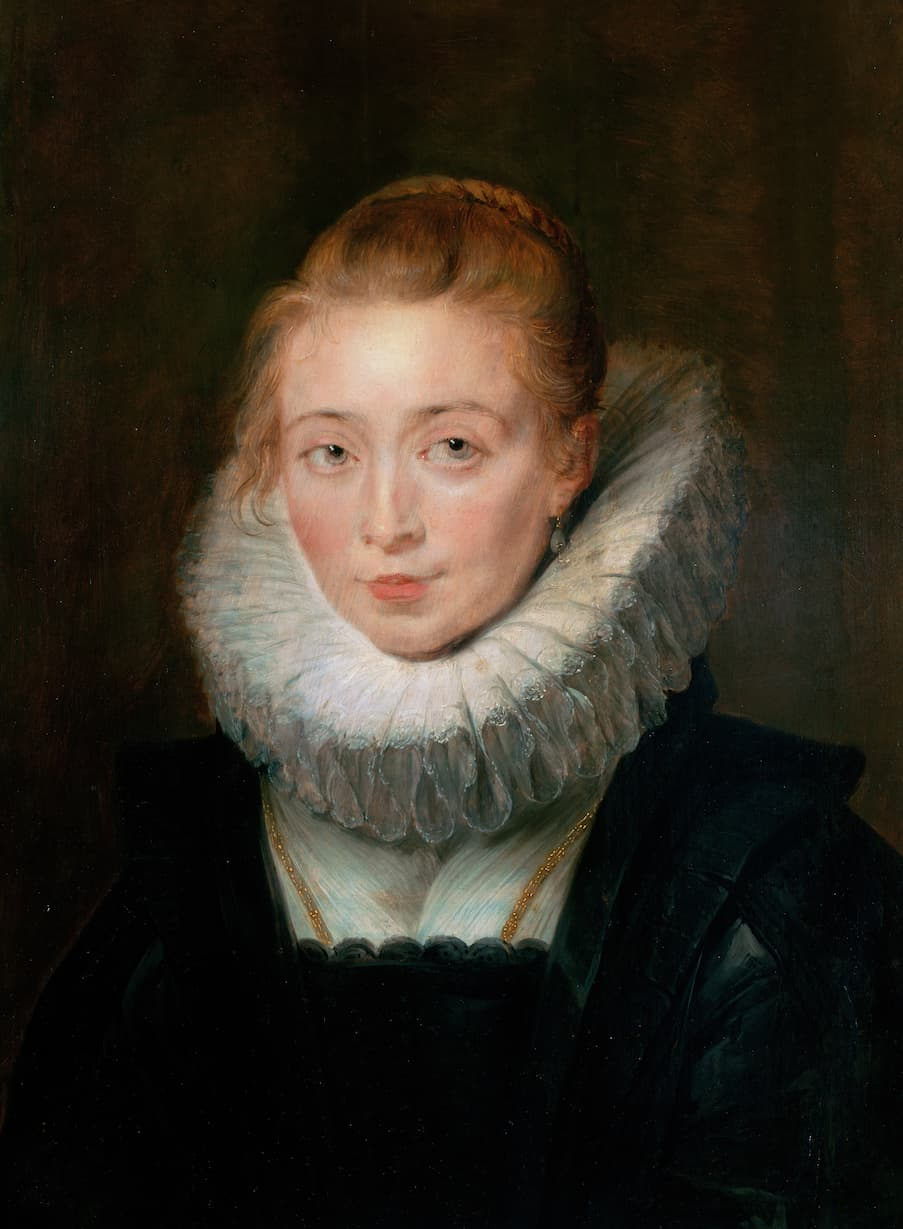
\includegraphics[width=0.5\linewidth]{img/test}
\caption{П. П. Рубенс «Портрет камеристки инфанты Изабеллы». Середина 1620-х гг. Эрмитаж, Санкт-Петербург}
\label{fig:test}
\end{figure}


\gostheading{Заключение}

Цели, поставленные во введении, достигнуты. Задачи выполнены. Результаты получены.

\gostheading{Список использованных источников}

\begin{thebibliography}{99}
	
\bibitem{ivanov2020} 
Иванов, И. И. Название книги : учебное пособие / И. И. Иванов, П. П. Петров. --- Москва : Издательство, 2020. --- 100 с. --- ISBN 978-5-00000-000-0. --- Текст : непосредственный.

\bibitem{petrov2021} 
Петров, С. С. Название статьи в журнале / С. С. Петров // Название журнала. --- 2021. --- Т. 1, № 2. --- С. 10--15. --- Текст : непосредственный.

\end{thebibliography}

\gostappendix{Пример заголовка приложения}

\section{Раздел приложения}

\subsection{Подраздел приложения}

Текст приложения

\begin{table}[h]
\caption{Название таблицы}\label{table2}
\resizebox{\textwidth}{!}{%
\begin{tabular}{|l|l|l|l|}
\hline
Заголовок столбца 1 & Заголовок столбца 2 & Заголовок столбца 3 & Заголовок столбца 4 \\ \hline
Заголовок строки    & Текст/Данные        & Текст/Данные        & Текст/Данные        \\ \hline
Заголовок строки    & Текст/Данные        & Текст/Данные        & Текст/Данные        \\ \hline
\end{tabular}%
}
\end{table}

\gostappendix{Пример листинга кода}

\VerbatimInput[
firstline=6,
lastline=15,
fontsize=\small,
breaklines=true,
numbers=left
]{preamble_gost.tex}

\VerbatimInput[
firstline=32,
lastline=44,
fontsize=\small,
breaklines=true,
numbers=left
]{preamble_gost.tex}

\gostappendix{Титульные листы ГУАП}

\include{title-pages/title_guap_coursework}

\include{title-pages/title_guap_laboratory}

%%% Титульный лист ГУАП для лабораторных работ
%%% Артемий Владин
%%% https://github.com/temavladin


%% Отключил нумерацию этой страницы
\thispagestyle{empty}

%% Установил 12-ый шрифт для этой страницы
\begingroup
\fontsize{12}{14.4}\selectfont


\begin{center}
ГУАП

\vspace{8mm}

КАФЕДРА \MakeUppercase{\setUniversityDepartment}
\end{center}

\vspace{13mm}

\begin{flushleft}
ОТЧЕТ
	
ЗАЩИЩЕН С ОЦЕНКОЙ
	
ПРЕПОДАВАТЕЛЬ
\end{flushleft}

\noindent \resizebox{\textwidth}{!}{%
\begin{tabular}{ccccc}
\hspace{5cm} & \hspace{0.25cm} & \hspace{4.5cm} & \hspace{0.25cm} & \hspace{4.5cm} \\
\setTeacherPosition & & & & \setTeacherName \\ \cline{1-1} \cline{3-3} \cline{5-5} 
{\fontsize{9}{12}\selectfont должность, уч. степень, звание} & & 
{\fontsize{9}{12}\selectfont подпись, дата} & & 
{\fontsize{9}{12}\selectfont инициалы, фамилия}
\end{tabular}
}

\vspace{7mm}

\begin{center}
{\fontsize{14}{18}\selectfont
ОТЧЕТ О ЛАБОРАТОРНОЙ РАБОТЕ \setWorkNumber
}
	
\vspace{12mm}
	
{\fontsize{14}{18}\selectfont \MakeUppercase{\setWorkName}}
\end{center}

\vspace{3mm}

\begin{center}
по курсу: \setUniversityDiscipline
\end{center}

\vfill

\begin{flushleft}
РАБОТУ ВЫПОЛНИЛ
\end{flushleft}

\noindent \resizebox{\textwidth}{!}{%
\begin{tabular}{@{}lccccc}
Студент гр. № & \setStudentGroup & & \hspace{2cm} \setDATE & & \setStudentName \\ \cline{2-2} \cline{4-4} \cline{6-6}
& & & 
{\fontsize{9}{12}\selectfont подпись, дата} & & 
{\fontsize{9}{12}\selectfont инициалы, фамилия} \\
\hspace{2.83cm} & \hspace{2cm} & \hspace{0.25cm} & \hspace{4cm} & \hspace{0.25cm} & \hspace{5cm} \\
\end{tabular}
}

\vspace{1.2 cm}

\begin{center}
Санкт-Петербург \the\year{}
\end{center}

\endgroup

%%% Титульный лист ГУАП для практических работ
%%% Артемий Владин
%%% https://github.com/temavladin


%% Отключил нумерацию этой страницы
\thispagestyle{empty}

%% Установил 12-ый шрифт для этой страницы
\begingroup
\fontsize{12}{14.4}\selectfont


\begin{center}
МИНИСТЕРСТВО НАУКИ И ВЫСШЕГО ОБРАЗОВАНИЯ РОССИЙСКОЙ ФЕДЕРАЦИИ
	
\vspace{0.5ex}
	
\scalebox{0.97}{Федеральное государственное автономное образовательное учреждение высшего образования}
	
«Санкт-Петербургский государственный университет аэрокосмического приборостроения»
	
\vspace{0.9cm}
	
КАФЕДРА \MakeUppercase{\setUniversityDepartment}
\end{center} 

\vspace{1.2cm}

\begin{flushleft}
ОТЧЕТ
	
ЗАЩИЩЕН С ОЦЕНКОЙ
	
ПРЕПОДАВАТЕЛЬ
\end{flushleft}

\noindent \resizebox{\textwidth}{!}{%
\begin{tabular}{ccccc}
\hspace{5cm} & \hspace{0.25cm} & \hspace{4.5cm} & \hspace{0.25cm} & \hspace{4.5cm} \\
\setTeacherPosition & & & & \setTeacherName \\ \cline{1-1} \cline{3-3} \cline{5-5} 
{\fontsize{9}{12}\selectfont должность, уч. степень, звание} & & 
{\fontsize{9}{12}\selectfont подпись, дата} & & 
{\fontsize{9}{12}\selectfont инициалы, фамилия}
\end{tabular}
}

\vspace{1.2cm}

\begin{center}
{\fontsize{14}{18}\selectfont
ОТЧЕТ
		
О ПРАКТИЧЕСКОЙ РАБОТЕ \setWorkNumber
}
	
\vspace{12mm}
	
{\fontsize{14}{18}\selectfont \MakeUppercase{\setWorkName}}
\end{center}

\vspace{3mm}

\begin{center}
по дисциплине: \setUniversityDiscipline
\end{center}

\vfill

\begin{flushleft}
РАБОТУ ВЫПОЛНИЛ
\end{flushleft}

\noindent \resizebox{\textwidth}{!}{%
\begin{tabular}{@{}lccccc}
Студент гр. № & \setStudentGroup & & \hspace{2cm} \setDATE & & \setStudentName \\ \cline{2-2} \cline{4-4} \cline{6-6}
& & & 
{\fontsize{9}{12}\selectfont подпись, дата} & & 
{\fontsize{9}{12}\selectfont инициалы, фамилия} \\
\hspace{2.83cm} & \hspace{2cm} & \hspace{0.25cm} & \hspace{4cm} & \hspace{0.25cm} & \hspace{5cm} \\
\end{tabular}
}

\vspace{1.2 cm}

\begin{center}
Санкт-Петербург \the\year{}
\end{center}

\endgroup

\end{document}